\section{App Features}

In the process of developing the application, we made several key design decisions to ensure efficiency, ease of use, and robust functionality. This subsection outlines the libraries and tools chosen for the graphical user interface (GUI) and database management, and presents the technical details and components of our user interface.

\subsection{Graphical User Interface: Tkinter and CustomTkinter}

The application's graphical user interface (GUI) has been meticulously crafted using the powerful \texttt{Tkinter} library, a standard Python interface to the Tk GUI toolkit. \texttt{Tkinter} is widely recognized for its simplicity and seamless integration with Python applications, offering an object-oriented interface that simplifies the development of responsive GUI applications.

In addition to \texttt{Tkinter}, the application leverages the enhanced capabilities of \texttt{CustomTkinter} to further elevate its visual appeal and functionality. \texttt{CustomTkinter} extends the features of \texttt{Tkinter} by providing advanced customization and theming options, including support for color modes, stylish switches, and dynamic menus. Through the seamless integration of \texttt{Tkinter} and \texttt{CustomTkinter}, the application not only delivers robust performance but also boasts a modern, user-friendly interface that enhances the overall user experience.

\subsection{Database Management: SQLite}

The application utilizes SQLite, a lightweight and self-contained SQL database engine, for database management. SQLite is integrated into Python through the \texttt{sqlite3} module, which offers a straightforward interface for database operations. We opted for SQLite due to its reliability, serverless nature, and zero-configuration database solution, making it ideal for our application.

SQLite's simplicity and ease of organization are its primary advantages. It stores the entire database in a single file on the disk, ensuring high portability and easy management. Given that our stored data isn't highly complex, SQLite was the perfect choice for us.

In Python, the \texttt{sqlite3} module enables efficient execution of SQL queries, management of database connections, and handling of transactions. This makes SQLite an optimal choice for applications that require a robust database solution without the overhead of a full-fledged database server.

By leveraging \texttt{Tkinter}, \texttt{CustomTkinter}, and SQLite, the application attains a harmonious blend of functionality, performance, and user experience.

\subsection{Technical Details}

The app is designed to enhance speech using the user's reference audio. Upon first use, the client must provide their name and upload a clear voice audio from their local device.

Afterward, the client needs to select the input device for real-time voice enhancement.

Additionally, the client can adjust the percentage of noise to be removed using the dry/wet slider.

Our app supports multiple users, each mapped to one reference audio. If a user needs to replace their reference audio, they can upload a new audio file, which will replace the old one.

Once these settings have been configured, the user will be able to activate the 'Cancel Noise' switch to start noise cancellation. Switching on disables other components, as the user is not allowed to modify their values while the app is running.

If the user deactivate the 'Cancel Noise' switch, the components are enabled again and noise cancellation is halted until the user edits their necessary data and clicks activate the switch again to resume.

Finally, the app is available in both light and dark modes to suit user preferences.

\begin{figure}[h]
	\centering
	\begin{minipage}{0.45\textwidth}
		\centering
		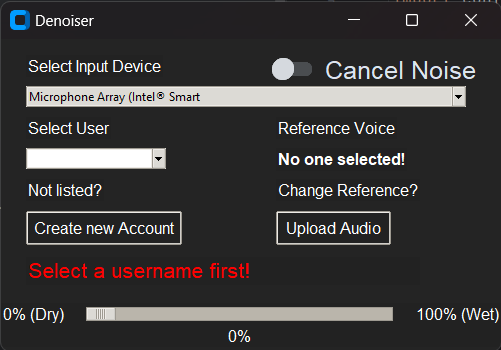
\includegraphics[width=\textwidth]{images/application/app_dark_mode.png}
		\label{fig:dark_mode}
	\end{minipage}\hfill
	\begin{minipage}{0.45\textwidth}
		\centering
		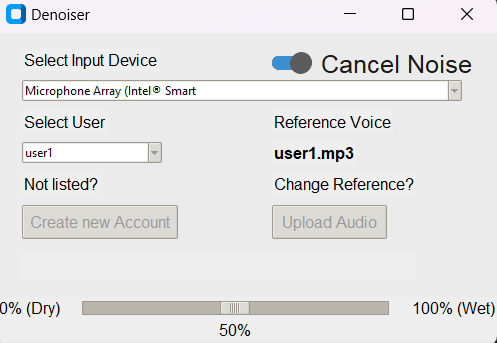
\includegraphics[width=\textwidth]{images/application/app_light_mode.png}
		\label{fig:light_mode}
	\end{minipage}
	\caption{Figure showing the appearance of our GUI in both: dark \& light mode}
	\label{fig:app_modes}
\end{figure}

Here is a recap of the features or components provided by our GUI:
\begin{itemize}
	\item \textbf{Select Input Device}: Dropdown menu that displays current audio inputs from the device.
	\item \textbf{Select User}: A dropdown menu that displays current saved usernames on the device. Once a user is selected, their reference voice's name appears next to the menu in bold.
	\item \textbf{Reference Voice}: Label that displays the user's reference audio once a user is chosen from the 'Select User' dropdown.
	\item \textbf{Create New Account}: Button that leads to another window, allowing the user to provide their name and upload their reference audio for the first time. Once this data is submitted, the user's name and reference audio remain saved in the app.
	\item \textbf{Upload Audio}: Button that enables a user to change their stored reference audio by uploading a new one.
	\item \textbf{Dry/Wet Slider}: Controls the amount of noise to keep or remove from the provided audio.
	\item \textbf{Cancel Noise}: Switch button that can be toggled on and off, initial state is 'off' while turning it on passes the given values to the model to start working.
\end{itemize}
